\documentclass[a4paper,14pt, unknownkeysallowed]{extreport}

\usepackage{cmap} % Улучшенный поиск русских слов в полученном pdf-файле
\usepackage[T2A]{fontenc} % Поддержка русских букв
\usepackage[utf8]{inputenc} % Кодировка utf8
\usepackage[english,russian]{babel} % Языки: русский, английский
\usepackage{enumitem}


\usepackage{threeparttable}

\usepackage[14pt]{extsizes}

\usepackage{caption}
\captionsetup{labelsep=endash}
\captionsetup[figure]{name={Рисунок}}

% \usepackage{ctable}
% \captionsetup[table]{justification=raggedleft,singlelinecheck=off}

\usepackage{amsmath}

\usepackage{geometry}
\geometry{left=30mm}
\geometry{right=10mm}
\geometry{top=20mm}
\geometry{bottom=20mm}

\usepackage{titlesec}
\titleformat{\section}
	{\normalsize\bfseries}
	{\thesection}
	{1em}{}
\titlespacing*{\chapter}{0pt}{-30pt}{8pt}
\titlespacing*{\section}{\parindent}{*4}{*4}
\titlespacing*{\subsection}{\parindent}{*4}{*4}

\usepackage{setspace}
\onehalfspacing % Полуторный интервал

\frenchspacing
\usepackage{indentfirst} % Красная строка

\usepackage{titlesec}
\titleformat{\chapter}{\LARGE\bfseries}{\thechapter}{20pt}{\LARGE\bfseries}
\titleformat{\section}{\Large\bfseries}{\thesection}{20pt}{\Large\bfseries}

\usepackage{multirow}
\usepackage{listings}
\usepackage{xcolor}

% Для листинга кода:
\lstset{%
	language=python,   					% выбор языка для подсветки	
	basicstyle=\small\sffamily,			% размер и начертание шрифта для подсветки кода
	numbers=left,						% где поставить нумерацию строк (слева\справа)
	%numberstyle=,						% размер шрифта для номеров строк
	stepnumber=1,						% размер шага между двумя номерами строк
	numbersep=5pt,						% как далеко отстоят номера строк от подсвечиваемого кода
	frame=single,						% рисовать рамку вокруг кода
	tabsize=4,							% размер табуляции по умолчанию равен 4 пробелам
	captionpos=t,						% позиция заголовка вверху [t] или внизу [b]
	breaklines=true,					
	breakatwhitespace=true,				% переносить строки только если есть пробел
	escapeinside={\#*}{*)},				% если нужно добавить комментарии в коде
	backgroundcolor=\color{white},
}


\usepackage{pgfplots}
\usetikzlibrary{datavisualization}
\usetikzlibrary{datavisualization.formats.functions}

\usepackage{graphicx}
\newcommand{\img}[3] {
	\begin{figure}[h!]
		\center{\includegraphics[height=#1]{img/#2}}
		\caption{#3}
		\label{img:#2}
	\end{figure}
}


\usepackage[justification=centering]{caption} % Настройка подписей float объектов

\usepackage[unicode,pdftex]{hyperref} % Ссылки в pdf
\hypersetup{hidelinks}

\usepackage{csvsimple}

\newcommand{\code}[1]{\texttt{#1}}





\begin{document}


\begin{titlepage}
	\newgeometry{pdftex, left=2cm, right=2cm, top=2.5cm, bottom=2.5cm}
	\fontsize{12pt}{12pt}\selectfont
	\noindent \begin{minipage}{0.15\textwidth}
		
\includegraphics[width=\linewidth]{img/b_logo.jpg}
	\end{minipage}
	\noindent\begin{minipage}{0.9\textwidth}\centering
		\textbf{Министерство науки и высшего образования Российской Федерации}\\
		\textbf{Федеральное государственное бюджетное образовательное учреждение высшего образования}\\
		\textbf{«Московский государственный технический университет имени Н. Э.~Баумана}\\
		\textbf{(национальный исследовательский университет)»}\\
		\textbf{(МГТУ им. Н. Э.~Баумана)}
	\end{minipage}
	
	\noindent\rule{18cm}{3pt}
	\newline\newline
	\noindent ФАКУЛЬТЕТ $\underline{\text{«Информатика и системы управления»~~~~~~~~~~~~~~~~~~~~~~~~~~~~~~~~~~~~~~~~~~~~~~~~~~~~~~~}}$ \newline\newline
	\noindent КАФЕДРА $\underline{\text{«Программное обеспечение ЭВМ и информационные технологии»~~~~~~~~~~~~~~~~~~~~~~~}}$\newline\newline\newline\newline\newline\newline\newline
	
	
	\begin{center}
		\noindent\begin{minipage}{1.3\textwidth}\centering
		\Large\textbf{   ~~~ Лабораторная работа №1}\newline
		\textbf{по дисциплине "Анализ Алгоритмов"}\newline\newline\newline
		\end{minipage}
	\end{center}
	
	\noindent\textbf{Тема} 			$\underline{\text{Расстояние Левенштейна и Дамерау-Левенштейна}}$\newline\newline
	\noindent\textbf{Студент} 		$\underline{\text{Ковалец К. Э.}}$\newline\newline
	\noindent\textbf{Группа} 		$\underline{\text{ИУ7-53Б}}$\newline\newline
	\noindent\textbf{Преподаватель} $\underline{\text{Волкова Л. Л.}}$\newline
	
	\begin{center}
		\vfill
		Москва~---~\the\year
		~г.
	\end{center}
	\restoregeometry
\end{titlepage}



\renewcommand{\contentsname}{Содержание} 
\tableofcontents
\setcounter{page}{2}





\chapter*{Введение}
\addcontentsline{toc}{chapter}{Введение}

В данной рабораторной работе будет рассмотрено расстояние Левенштейна. Данное расстояние показывает минимальное количество операций (вставки, удаления, замены), которое необходимо для перевода одной строки в другую. Это расстояние помогает определить схожесть двух строк.

Расстояние Левенштейна применяется в теории информации и компьютерной лингвистике для:

\begin{itemize}
	\item исправления ошибок в слове;
	\item сравнения текстовых файлов утилитой diff;
	\item для сравнения генов, хромосом и белков в биоинформатике.
\end{itemize}

Целью данной лабораторной работы является изучение и применение метода динамического программирования на материале алгоритмов Левенштейна и Дамерау-Левенштейна, а также получение практических навыков реализации указанных алгоритмов. Для достижения поставленной цели необходимо выполнить следующие задачи:

\begin{itemize}
	\item изучить расстояния Левенштейна и Дамерау-Левенштейна;
	\item реализовать указвнные алгоритмы поиска расстояний (два алгоритма в матричной версии и один из алгоритмов в рекурсивной версии)
	\item примененить метод динамического программирования для матричной реализации указанных алгоритмов; 
	\item провести сравнительный анализ линейной и рекурсивной реализаций алгоритмов по затраченному процессорному времени и памяти на основе экспериментальных данных;
	\item описать и обосновать полученные результаты в отчете о выполненной лабораторной работе.
\end{itemize}





\chapter{Аналитическая часть}

В данном разделе будут рассмотрены алгоритмы нахождения расстояний Левенштейна и Дамерау-Левенштейна.

\section{Расстояние Левенштейна}

Расстояние Левенштейна [1] ~--~ это минимальное количество операций вставки, удаления и замены, необходимох для превращения одной строки в другую.

Цены операций могут зависеть от вида операций (вставка, удаление, замена) и/или от участвующих в ней символов, отражая разную вероятность разных ошибок при вводе текста и т.п. В общем случае

\begin{itemize}
	\item $w(a, b)$ ~--~ цена замены символа $a$ на $b$, R (от англ. replace);
	\item $w(\lambda, b)$ ~--~ цена вставки символа $b$, I (от англ. insert);
	\item $w(a, \lambda)$ ~--~ цена удаления символа $a$, D (от англ. delete).
\end{itemize}

Для решения задачи о редакционном расстоянии необходимо найти последовательность замен, минимизирующую суммарную цену. Расстояние Левенштейна является частным случаем этой задачи при

\begin{itemize}
	\item $w(a, a) = 0$;
	\item $w(a, b) = 1$, $a \neq b$;
	\item $w(\lambda, b) = 1$;
	\item $w(a, \lambda) = 1$.
\end{itemize}

Имеем две строки $S_{1}$ и $S_{2}$, длинной M и N соответственно. Расстояние Левенштейна рассчитывается по рекуррентной формуле формуле \ref{eq:L}:

\begin{equation}
	\label{eq:L}
	D(i, j) = \begin{cases}
	0, &\text{i = 0, j = 0}\\
	i, &\text{j = 0, i > 0}\\
	j, &\text{i = 0, j > 0}\\
	min \begin{cases}
		D(i, j - 1) + 1\\
		D(i - 1, j) + 1\\
		D(i - 1, j - 1) + m(S_{1}[i], S_{2}[i]) \\
	\end{cases}
	&\text{i > 0, j > 0}
	\end{cases}
\end{equation}

\vspace{5mm}

где функция \ref{eq:m} определена как:
\begin{equation}
\label{eq:m}
m(a, b) = \begin{cases}
0 &\text{если a = b,}\\
1 &\text{иначе}
\end{cases}.
\end{equation}


Рекурсивный алгоритм реализует формулу \ref{eq:L}. Функция $D$ составлена таким образом, что для перевода из строки $a$ в строку $b$ требуется выпол- нить последовательно некоторое количество операций (удаление, вставка, замена) в некоторой последовательности. Полагая, что $a'$, $b'$ — строки $a$ и $b$ без последнего символа соответственно, цена преобразования из строки $a$ в строку $b$ может быть выражена как:

\begin{itemize}
	\item сумма цены преобразования строки $a'$ в $b'$ и цены проведения операции удаления, которая необходима для преобразования $a'$ в $a$;
	\item сумма цены преобразования строки $a$ в $b'$ и цены проведения операции вставки, которая необходима для преобразования $b'$ в $b$;
	\item сумма цены преобразования из $a'$ в $b'$ и операции замены, предполагая, что $a$ и $b$ оканчиваются на разные символы;
	\item цена преобразования из $a'$ в $b'$, предполагая, что $a$ и $b$ оканчиваются на один и тот же символ.
\end{itemize}

Минимальной ценой преобразования будет минимальное значение приведенных вариантов.

\section{Расстояние Дамерау-Левенштейна}

В алгоритме поиска расстояния Дамерау-Левенштейна, помимо вставки, удаления, и замены присутствует  еще одна редакторская операция - транспозиция T (от англ. transposition).

Расстояние Дамерау-Левенштейна может быть вычисленно по рекуррентной формуле \ref{eq:DL}:

\begin{equation}
	\label{eq:DL}
	D(i, j) = \begin{cases}
	0 \qquad\qquad\qquad\qquad\qquad\qquad\qquad\qquad\qquad ,j = 0, i = 0\\
	i \qquad\qquad\qquad\qquad\qquad\qquad\qquad\qquad\qquad ,j = 0, i > 0\\
	j \qquad\qquad\qquad\qquad\qquad\qquad\qquad\qquad\qquad ,j > 0, i = 0\\
	min \begin{cases}
		D(i, j - 1) + 1\\
		D(i - 1, j) + 1\\
		D(i - 1, j - 1) + m(S_{1}[i], S_{2}[i]) \\
		D(i - 2, j - 2) + m(S_{1}[i], S_{2}[i]) \\
	\end{cases}
	\begin{aligned}
		& , \text{если i > 1, j > 1} \\
		& , S_{1}[i] = S_{2}[j - 1]  \\
		& , S_{1}[j] =  S_{2}[i - 1] \\
	\end{aligned}\\
	min \begin{cases}
		D(i, j - 1) + 1\\
		D(i - 1, j) + 1 & \;\; \text{,иначе}\\
		D(i - 1, j - 1) + m(S_{1}[i], S_{2}[i]) \\
	\end{cases}
	\end{cases}
\end{equation}
	    
\section{Вывод}
В данном разделе были рассмотрены алгоритмы нахождения расстояния Левенштейна и Дамерау-Левенштейна,
формулы которых задаются реккурентно, а следовательно, данные алгоритмы могут быть реализованы рекурсивно и итерационно. На вход алгоритмам будут поступать две строки, которые могут содержать как русские, так и английские буквы, также будет предусмотрен ввод пустых строк. Реализуемое ПО будет давать возможность выбрать алгоритм и вывести для него результат вычисления, а также возможность произвести сравнение алгоритмов по затраченному времени.





\chapter{Конструкторская часть}
В данном разделе будут приведены схемы алгоритмов нахождения расстояний Левенштейна и Дамерау-Левенштейна, приведено описание используемых типов данных, оценки памяти, а также описана структура ПО.

\section{Схемы алгоритмов}

На вход алгоритмов падаются строки s1 и s2, на выходе получаем едиственное число - искомое расстояние.

На рис. \ref{fig:L_rec} - \ref{fig:DL_table} приведены схемы рекурсивных и матричных алгоритмов Левенштейна и Дамерау-Левенштейна.

\clearpage

\begin{figure}[h]
	\centering
	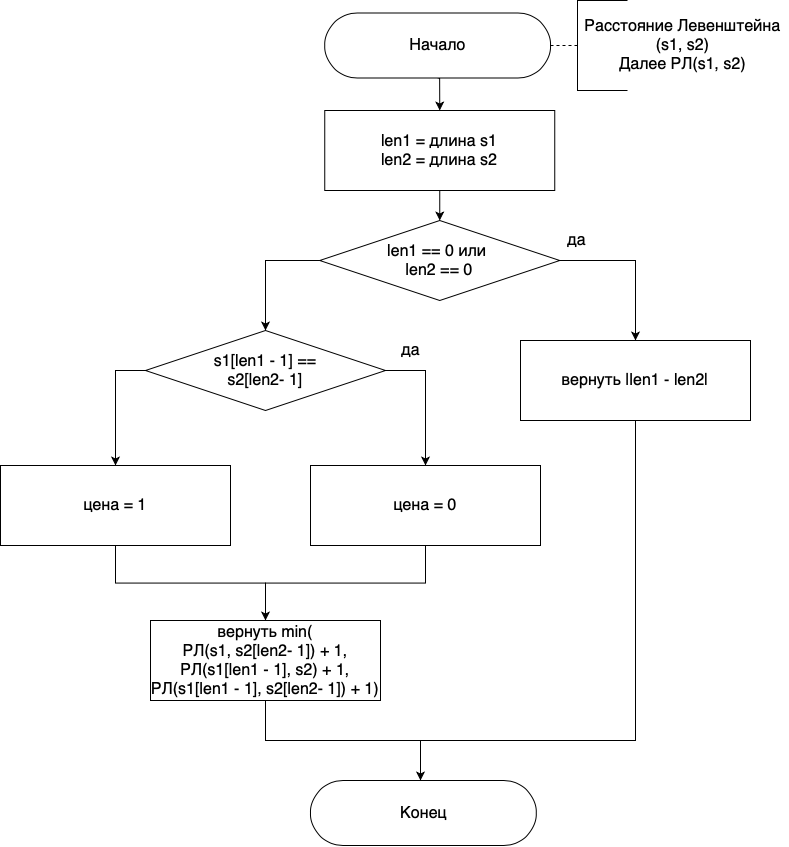
\includegraphics[scale=0.6]{img/lev_recursion_scheme.png}
	\caption{Схема рекурсивного алгоритма нахождения расстояния Левенштейна}
	\label{fig:L_rec}
\end{figure}

\clearpage

\begin{figure}[h]
	\centering
	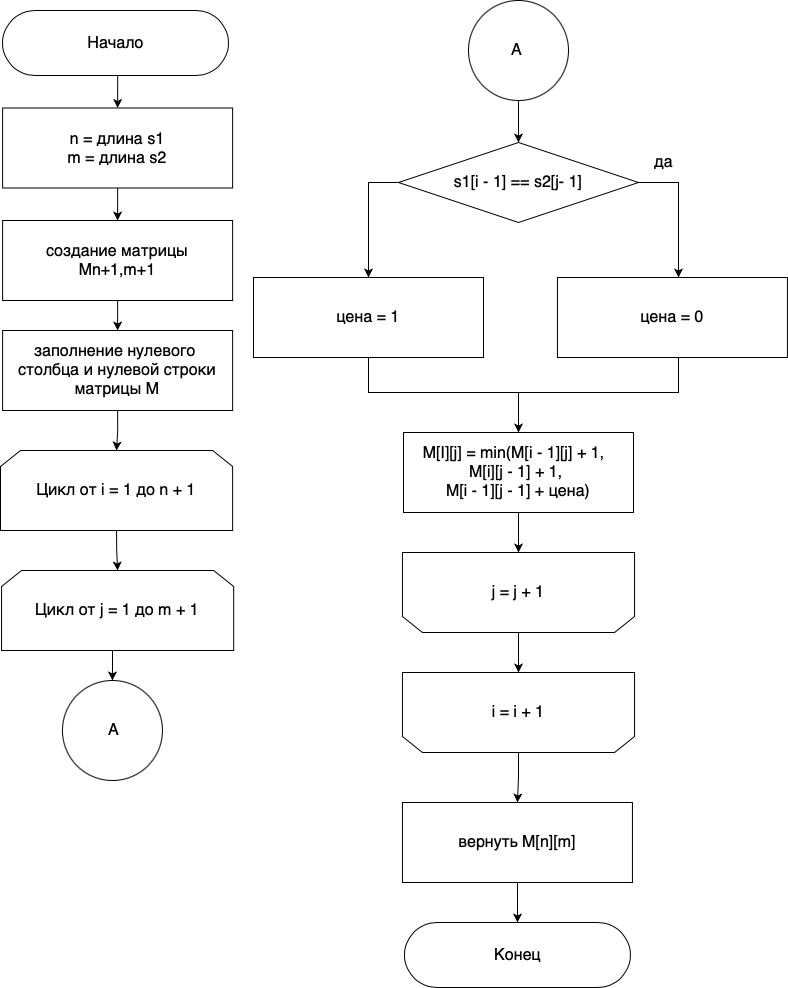
\includegraphics[scale=0.6]{img/lev_table_scheme.png}
	\caption{Схема матричного алгоритма нахождения расстояния Левенштейна}
	\label{fig:L_table}
\end{figure}

\clearpage

\begin{figure}[h]
	\centering
	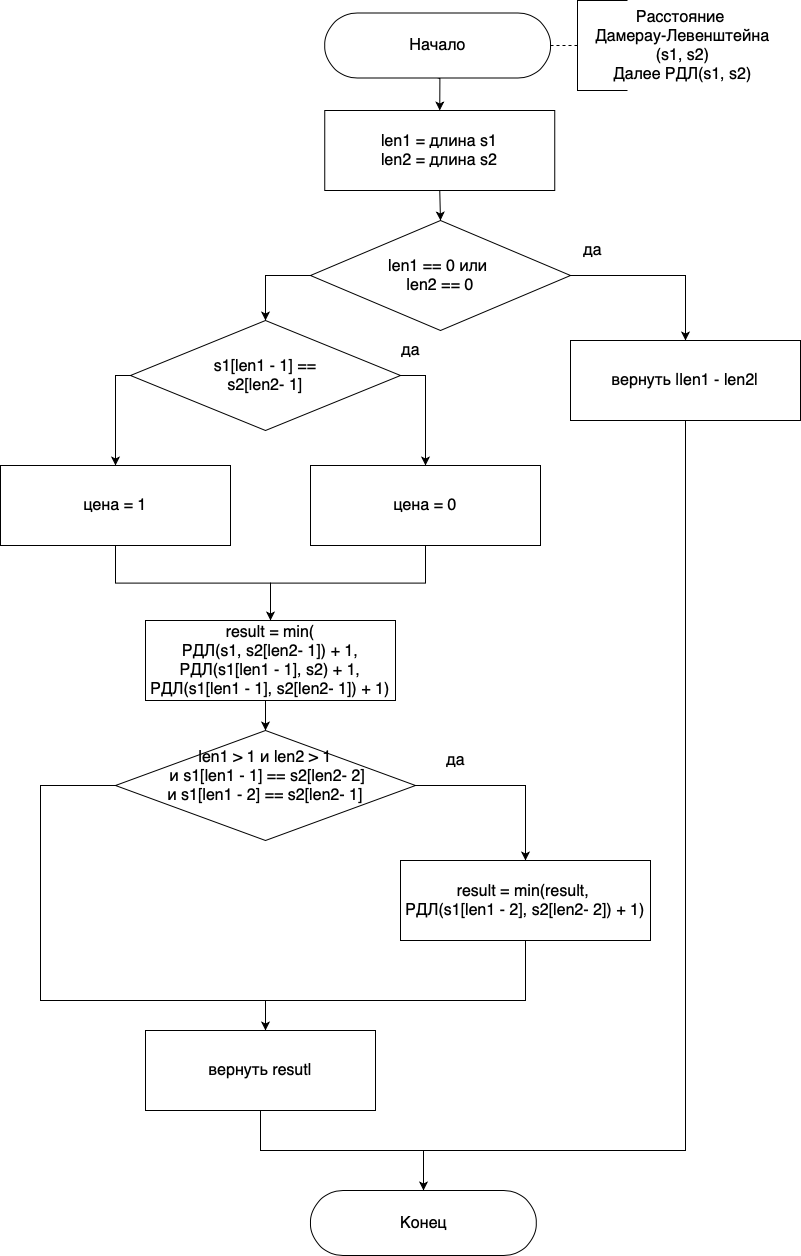
\includegraphics[scale=0.55]{img/dam_lev_recursion_scheme.png}
	\caption{Схема рекурсивного алгоритма нахождения расстояния Дамерау-Левенштейна}
	\label{fig:DL_rec}
\end{figure}

\clearpage

\begin{figure}[h]
	\centering
	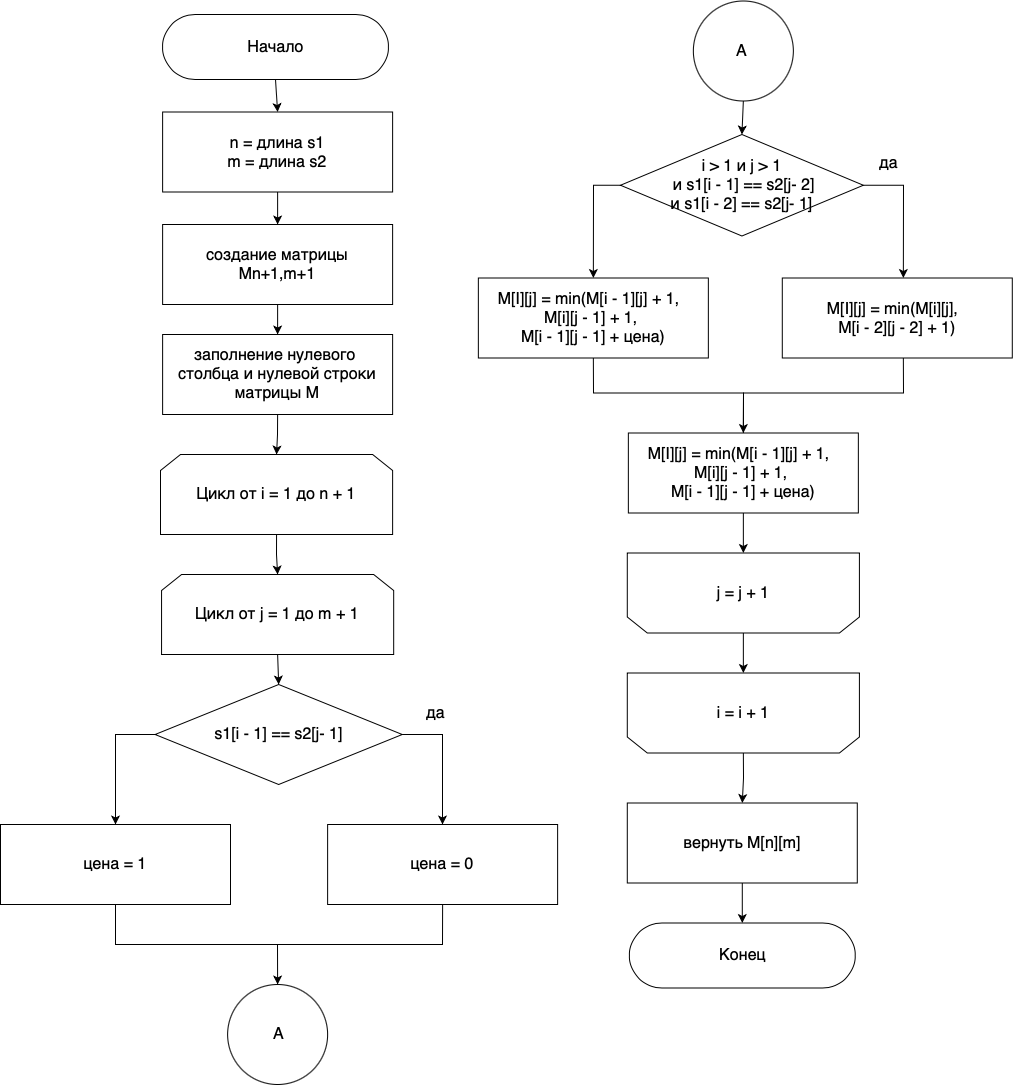
\includegraphics[scale=0.48]{img/dam_lev_table_scheme.png}
	\caption{Схема матричного алгоритма нахождения расстояния Дамерау-Левенштейна}
	\label{fig:DL_table}
\end{figure}

\clearpage

\section{Описание используемых типов данных}

При реализации алгоритмов будут использованы следующие структуры данных:

\begin{itemize}
	\item строка - массив типа $char$ размером длины строки;
	\item длина строки - целое число типа $int$;
	\item матрица - двумерный массив типа $int$.
\end{itemize}

\section{Оценка памяти}

Алгоритмы Левенштейна и Дамерау-Левенштейна не отличаются по использованию памяти, поэтому достаточно рассмотреть рекурсивную и матричную реализации одного из этих алгоритмов.

Максимальная глубина стека вызовов при рекурсивной реализации равна сумме длин входящих строк, а на каждый вызов функции требуется еще 3 дополнительных переменных типа \textit{int}, соответственно, максимальный расход памяти

\begin{equation}
	(Len(S_{1}) + Len(S_{2})) \cdot (2 \cdot Size(\text{string}) + 3 \cdot Size(\text{int})),
\end{equation}

\noindent
где $S_{1}, S_{2}$ - строки, Size - функция, возвращающая размер аргумента; Len - функция, возвращающая длину строки, string - строковый тип, int - целочисленный.

Использование памяти при итеративной реализации теоритически равно

\begin{equation}
	(Len(S_{1}) + 1) \cdot (Len(S_{2}) + 1) \cdot Size(int) + 3 \cdot Size(int) + 2 \cdot Size(string)
\end{equation}

По расходу памяти итеративные алгоритмы проигрывают рекурсивным: максимальный размер используемой памяти в них растёт как произведение длин строк, в то время как у рекурсивного алгоритма — как сумма длин строк.

\clearpage

\section{Классы эквивалентности}

Выделенные классы эквивалентности для тестирования:

\begin{itemize}
	\item ввод пустых строк;
	\item одна из строк - пустая;
	\item расстояния Левенштейна и Дамерау–Левенштейна равны;
	\item расстояния Левенштейна и Дамерау–Левенштейна различны;
\end{itemize}

\section{Структура ПО}

ПО будет состоять из следующих модулей:

\begin{itemize}
	\item $main.py$ - файл, содержащий функцию $main$;
    \item $algorithms.py$ - файл, содержащий код всех алгоритмов нахождения расстояния Левенштейна и Дамерау-Левенштейна;
    \item $compare\_time.py$ - файл, в котором содержатся функции для замера времени работы алгоритмов;
    \item $in\_out.py$ - файл, в котором содержатся функции ввода-вывода;
    \item $color.py$ - файл, который содержит переменные типа $string$ для цветного вывода результата работы программы в консоль.
\end{itemize}

\section{Вывод}

В данном разделе на основе теоретических данных были построены схемы требуемых алгоритмов, выбраны используемые типы данных, а также была проведена оценка затрачиваемого объёма памяти и описана структура ПО.

\clearpage





\chapter{Технологическая часть}

В данном разделе будут приведены требования к программному обеспечению, средства реализации, листинги кода, а также функциональные тесты.

\section{Требования к программному обеспечению}

\begin{itemize}
    \item входные данные - две строки на русском или английском языке в любом регистре;
    \item выходные данные - искомое расстояние для выбранного метода и матрицы расстояний для матричных реализаций.
\end{itemize}

\section{Средства реализации}
В данной работе для реализации был выбран язык программирования $Python$ [2]. Выбор обсуловлен наличием опыта работы с ним. Время работы было замерено с помощью функции \textit{process\_time} из библиотеки $time$ [3].





\section{Листинги кода}

В листингах \ref{lst:lev_recursion} - \ref{lst:dam_lev_table} представлены реализации алгоритмов нахождения расстояния Левенштейна и Дамерау–Левенштейна.

\clearpage

\begin{center}
\captionsetup{justification=raggedright,singlelinecheck=off}
\begin{lstlisting}[label=lst:lev_recursion,caption=Функция нахождения расстояния Левенштейна рекурсивно]
def lev_recursion(s1, s2, output = False):
    len1 = len(s1)
    len2 = len(s2)

    if len1 == 0 or len2 == 0:
        return abs(len1 - len2)

    m = 0 if s1[-1] == s2[-1] else 1

    return min(lev_recursion(s1,      s2[:-1]) + 1,
               lev_recursion(s1[:-1], s2     ) + 1,
               lev_recursion(s1[:-1], s2[:-1]) + m)
\end{lstlisting}
\end{center}


\begin{center}
\captionsetup{justification=raggedright,singlelinecheck=off}
\begin{lstlisting}[label=lst:lev_table,caption=Функция нахождения расстояния Левенштейна итеративно]
def lev_table(s1, s2, output = False):
    len1 = len(s1)
    len2 = len(s2)

    M = [[i + j for j in range(len2 + 1)] 
                for i in range(len1 + 1)]

    for i in range(1, len1 + 1):
        for j in range(1, len2 + 1):

            m = 0 if s1[i - 1] == s2[j - 1] else 1

            M[i][j] = min(M[i - 1][j    ] + 1,
                          M[i    ][j - 1] + 1,
                          M[i - 1][j - 1] + m)
    if output:  
        output_table(M, s1, s2)

    return M[-1][-1]
\end{lstlisting}
\end{center}

\clearpage

\begin{center}
\captionsetup{justification=raggedright,singlelinecheck=off}
\begin{lstlisting}[label=lst:dam_lev_recursion,caption=Функция нахождения расстояния Дамерау–Левенштейна рекурсивно]
def dam_lev_recursion(s1, s2, output = False):
    len1 = len(s1)
    len2 = len(s2)

    if len1 == 0 or len2 == 0:
        return abs(len1 - len2)

    m = 0 if s1[-1] == s2[-1] else 1

    result = min(dam_lev_recursion(s1,      s2[:-1]) + 1,
                 dam_lev_recursion(s1[:-1], s2     ) + 1,
                 dam_lev_recursion(s1[:-1], s2[:-1]) + m)

    if len1 > 1 and len2 > 1 and s1[-1] == s2[-2] \
                             and s1[-2] == s2[-1]:
        result = min(result, dam_lev_recursion(s1[:-2], s2[:-2]) + 1)

    return result
\end{lstlisting}
\end{center}

\clearpage

\begin{center}
\captionsetup{justification=raggedright,singlelinecheck=off}
\begin{lstlisting}[label=lst:dam_lev_table,caption=Функция нахождения расстояния Дамерау–Левенштейна итеративно]
def dam_lev_table(s1, s2, output = False):
	len1 = len(s1)
	len2 = len(s2)

	M = [[i + j for j in range(len2 + 1)] 
				for i in range(len1 + 1)]
	
	for i in range(1, len1 + 1):
		for j in range(1, len2 + 1):

			m = 0 if s1[i - 1] == s2[j - 1] else 1

			M[i][j] = min(M[i - 1][j    ] + 1,
						  M[i    ][j - 1] + 1,
						  M[i - 1][j - 1] + m)

			if i > 1 and j > 1 and s1[i - 1] == s2[j -2 ] \
							   and s1[i - 2] == s2[j - 1]:
				M[i][j] = min(M[i][j], M[i - 2][j - 2] + 1)

	if output:  
		output_table(M, s1, s2)

	return M[-1][-1]
\end{lstlisting}
\end{center}

\clearpage

\section{Функциональные тесты}

В таблице \ref{tbl:functional_test} приведены функциональные тесты для алгоритмов вычисления расстояния Левенштейна и Дамерау—Левенштейна. Все тесты пройдены успешно.

\begin{table}[h]
	\begin{center}
	\begin{threeparttable}
		\captionsetup{justification=raggedright,singlelinecheck=off}
		\caption{\label{tbl:functional_test} Функциональные тесты}
		\begin{tabular}{|c|c|c|c|}
			\hline
			\multirow{2}{*}{1-ая строка} & \multirow{2}{*}{2-ая строка} & \multicolumn{2}{c|}{Ожидаемый результат} \\ \cline{3-4} 
			&  & Левенштейн & Дамерау-Левенштейн 
			\\ \hline
			[]	       & []       & 0    & 0               
			\\ \hline
			[]	       & цветы    & 5    & 5               
			\\ \hline
			бегемот    & бегемот  & 0    & 0                
			\\ \hline
			скат       & кот      & 2    & 2                
			\\ \hline
			красивый   & карсивый & 2    & 1                   
			\\ \hline
			вагон      & гонки    & 4    & 4                   
			\\ \hline
			бар        & раб      & 2    & 2                   
			\\ \hline
			слон       & слоны    & 1    & 1                   
			\\ \hline
		\end{tabular}
	\end{threeparttable}
	\end{center}
\end{table}


\section{Вывод}

В данном разделе были разработаны алгоритмы поиска расстояний Левенштейна и Дамерау–Левенштейна (рекурсивные и с заполнением матрицы), а также проведено тестирование.





\chapter{Исследовательская часть}

\section{Технические характеристики}

Технические характеристики устройства, на котором выполнялось тестирование представлены далее.

\begin{itemize}
    \item Операционная система: macOS 11.5.2. [4]
    \item Память: 8 GiB.
    \item Процессор: 2,3 GHz 4‑ядерный процессор Intel Core i5. [5]
\end{itemize}

При тестировании ноутбук был включен в сеть электропитания. Во время тестирования ноутбук был нагружен только встроенными приложениями окружения, а также системой тестирования.

\section{Демонстрация работы программы}

\img{100mm}{example}{Пример работы программы}
\clearpage

\section{Время выполнения алгоритмов}

Результаты замеров времени работы алгоритмов нахождения расстояний Левенштейна и Дамерау–Левенштейна приведены в таблице \ref{tbl:time_measurements}. Замеры времени проводились на строках одинаковой длины и усреднялись для каждого набора одинаковых экспериментов.

\begin{table}[h]
	\begin{center}
		\begin{threeparttable}
		\captionsetup{justification=raggedright,singlelinecheck=off}
		\caption{Время работы алгоритмов (в секундах)}
		\label{tbl:time_measurements}
		\begin{tabular}{|c|c|c|c|c|}
			\hline
			Длина строк &  Лев рек.  & Дам-Лев рек. & Лев итер. & Дам-Лев итер. \\
			\hline
			1    & 5.64e-06 & 4.93e-06 & 2.60e-06 & 2.20e-06 \\ 
			\hline
			2    & 6.05e-06 & 7.61e-06 & 9.30e-06 & 9.30e-06 \\ 
			\hline
			3    & 9.85e-06 & 1.02e-05 & 4.39e-05 & 4.51e-05 \\ 
			\hline
			4    & 1.51e-05 & 1.61e-05 & 2.02e-04 & 2.07e-04 \\ 
			\hline
			5    & 2.08e-05 & 2.34e-05 & 1.09e-03 & 1.09e-03 \\ 
			\hline
			6    & 2.82e-05 & 3.22e-05 & 5.69e-03 & 5.83e-03 \\ 
			\hline
			7    & 3.67e-05 & 4.28e-05 & 3.07e-02 & 3.22e-02 \\ 
			\hline
			8    & 4.72e-05 & 5.48e-05 & 1.68e-01 & 1.73e-01 \\ 
			\hline
		\end{tabular}
		\end{threeparttable}
    \end{center}
\end{table}


\img{114mm}{time_measurements}{Сравнение алгоритмов по времени}
\clearpage


Наиболее эффективными являются алгоритмы, использующие матрицы, так как в рекурсивных алгоритмах большое количество повторных расчетов.

\section{Вывод}

Рекурсивные алгоритмы Левенштейна и Дамерау–Левенштейна работают на несколько порядков дольше реализаций, использующих матрицы (в 10 раз при длине строки - 4, в 100 раз при длине - 6 и в 1000 раз при длине строки - 8), время их работы увеличивается в геометрической прогрессии. Также стоит заметить, что как рекурсивные, так и итеративные алгоритмы сопостовимы между собой по времени выполнения и примерно равны.



 

\chapter*{Заключение}
\addcontentsline{toc}{chapter}{Заключение}

Было экспериментально подтверждено различие во временной эффективности рекурсивной и нерекурсивной реализаций выбранных алгоритмов нахождения расстояния между строками при помощи разработаного программного обеспечения на материале замеров процессорного времени выполнения реализаций на различных длинах строк. 

В результате исследований можно сделать вывод о том, что матричная реализация данных алгоритмов заметно выигрывает по времени при росте длин строк, но проигрывает по количеству затрачиваемой памяти.

\vspace{5mm}

В ходе выполнения данной лабораторной работы были решены следующие задачи:
\begin{itemize}
	\item изучены алгоритмов Левенштейна и Дамерау-Левенштейна нахождения расстояния между строками;
	\item применены методы динамического программирования для матричной реализации указанных алгоритмов;
	\item получены практические навыки реализации указанных алгоритмов: двух алгоритмов в матричной версии и одного из алгоритмов в рекурсивной версии;
	\item проведен сравнительный анализ линейной и рекурсивной реализаций выбранного алгоритма определения расстояния между строками по затрачиваемым ресурсам (времени и памяти);
	\item экспериментально подтверждено различие во временнoй эффективности рекурсивной и нерекурсивной реализаций выбранного алгоритма определения расстояния между строками при помощи разработанного программного обеспечения на материале замеров процессорного времени выполнения реализации на варьирующихся длинах строк;
	\item описаны и обоснованы полученные результаты в отчете о выполненной лабораторной работе, выполненного как расчётно-пояснительная записка к работе.
\end{itemize}




\begin{thebibliography}{5}
	\bibitem{bib1}
	Левенштейн В. И. Двоичные коды с исправлением выпадений, вставок и замещений символов. – М.: Доклады АН СССР, 1965. Т. 163. С. 845– 848.
	\bibitem{bib2}
	Welcome to Python [Электронный ресурс]. Режим доступа: \url{https://www.python.org} (дата обращения: 17.10.2021).
	\bibitem{bib3}
	time — Time access and conversions [Электронный ресурс]. Режим доступа: \url{https://docs.python.org/3/library/time.html#functions} (дата обращения: 17.10.2021).
	\bibitem{bib4}
	macOS Monterey - Apple(RU) [Электронный ресурс]. Режим доступа: \url{https://www.apple.com/ru/macos/monterey/} (дата обращения: 17.10.2021).
	\bibitem{bib5}
	Intel [Электронный ресурс]. Режим доступа: \url{https://www.intel.ru/content/www/ru/ru/products/details/processors/core/i5.html} (дата обращения: 17.10.2021).
\end{thebibliography}

\addcontentsline{toc}{chapter}{Список литературы}

\end{document}
